% Revisão OK 30/09
\chapter{Teste de Carga}

Para avaliar a confiabilidade do projeto em cenários extremos com muitos acessos 
simultâneos, utilizou-se a framework de testes Locust. A vantagem dessa ferramenta 
é que ela é uma biblioteca Python, permitindo que, com código Python, seja possível
escrever as chamadas "tasks" \cite{locust}, que são as requisições a serem feitas.
Cada task é uma função com um decorator Python específico.

Para aumentar a confiança nos testes, as rotas são chamadas com ICAOs aleatórios.

Para garantir que os testes consultassem exclusivamente o meu servidor, coloquei 
o Cloudflare no modo de desenvolvedor, o que desativa a função de cache.

\begin{figure}[ht]
    \begin{center}
    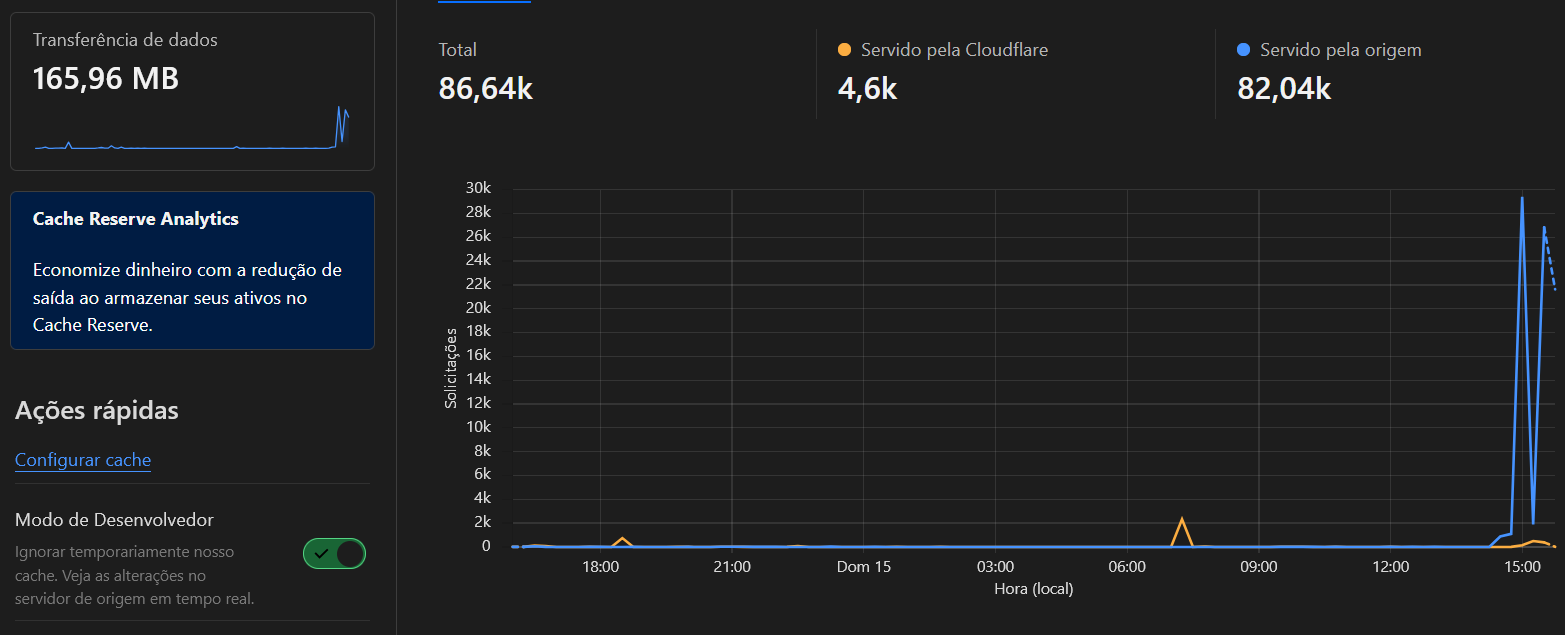
\includegraphics[width=400pt]{img/cloudflare-dev-mode.png}
    \caption{Cache no Cloudflare desativado. Note que a linha azul está bem acima 
    da linha laranja, mostrando que meu servidor de origem está servindo as requisições}
    \label{fig:cloudflare-dev-mode}
    \end{center}
\end{figure}

O maior gargalo deste projeto era o acesso ao banco de dados. Ao testar com 500 
usuários simultâneos, no pior caso, o tempo de resposta ultrapassava 15 segundos, 
o que é totalmente inaceitável para um código de produção.

\begin{figure}[ht]
    \begin{center}
    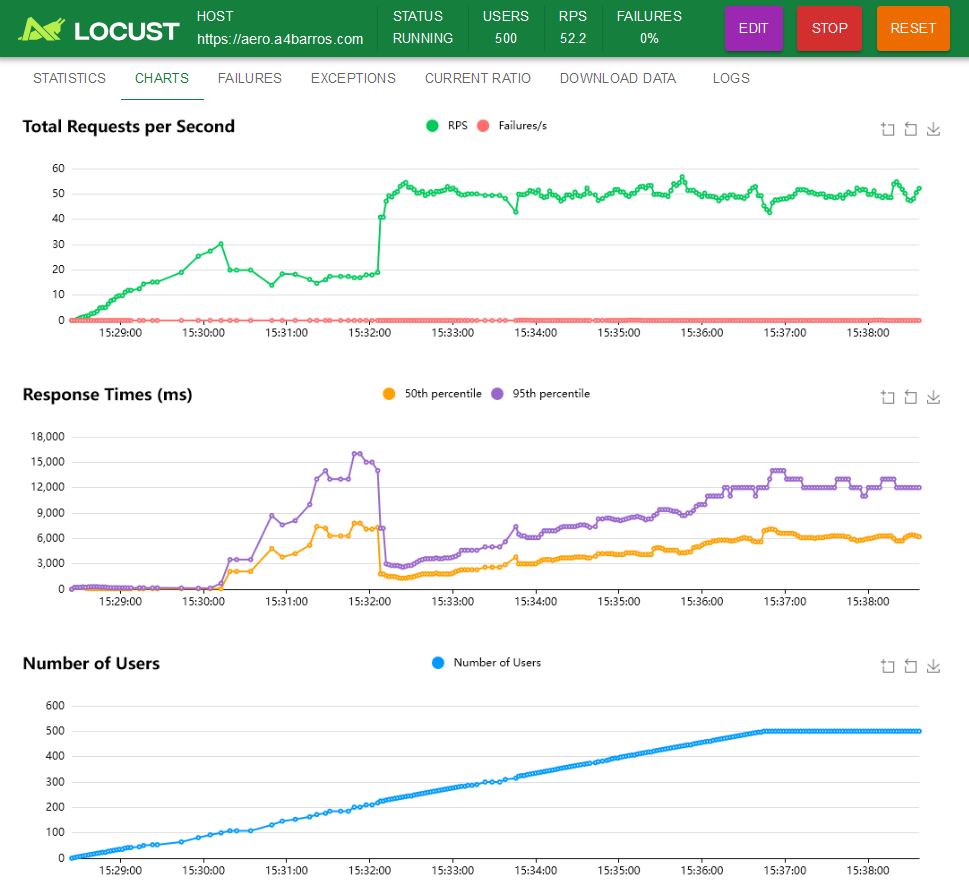
\includegraphics[width=400pt]{img/locust-no-cache.png}
    \caption{Teste de carga no Locust}
    \label{fig:locust-no-cache}
    \end{center}
\end{figure}


Uma ideia seria utilizar um banco de dados em memória, como o Redis, para fazer 
cache das respostas. No entanto, isso demandaria tempo de desenvolvimento. Então, 
pensei em uma forma de fazer cache da resposta completa. Existem bibliotecas que 
se integram com o FastAPI como middleware, e, ao adicionar um decorador antes da
definição da rota, é possível configurar um cache com o tempo definido pelo 
programador. Contudo, essas bibliotecas não estão sendo mantidas, o que traz o 
risco de pararem de funcionar sem aviso.

Devido a este risco, optei por uma solução mais declarativa, em vez de implementar
algo próprio.

Como já tenho o NGINX funcionando como proxy reverso, utilizei o próprio NGINX 
para realizar o cache das respostas. Configurei o cache com um tempo de um minuto, 
ou seja, no pior caso, a informação ficará desatualizada por até 1 minuto. Como 
o METAR é atualizado a cada hora, no pior cenário, alguém acessaria a página com 
o METAR às 17:59:59, e essa informação seria armazenada no cache. Às 18:00:00 
sairia um novo METAR, e apenas às 18:00:59 a informação seria atualizada, o que
 é aceitável, considerando o ganho de escala.

\begin{figure}[ht]
    \begin{center}
    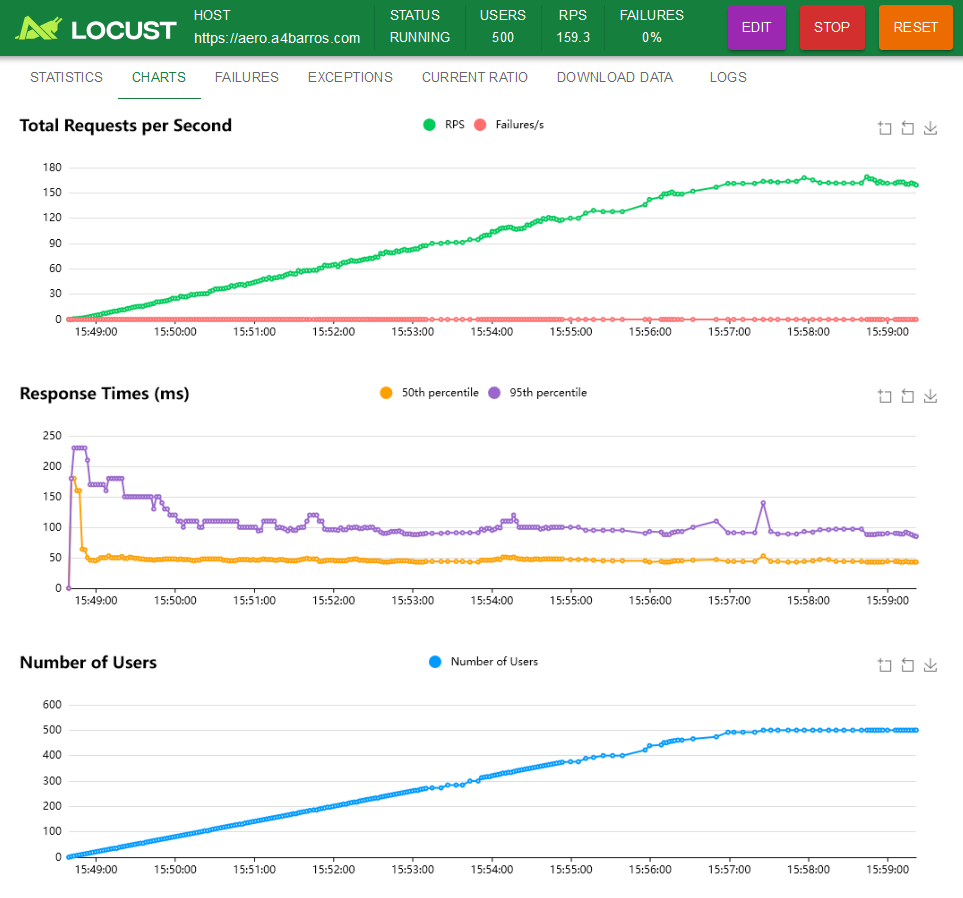
\includegraphics[width=400pt]{img/locust-cache.png}
    \caption{Teste de carga no Locust com cache do NGINX}
    \label{fig:locust-cache}
    \end{center}
\end{figure}